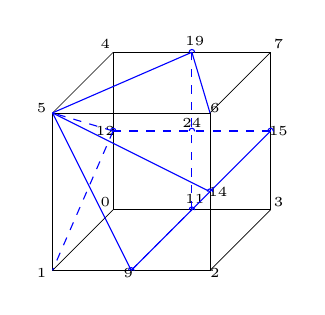
\begin{tikzpicture}
    %Pattern 10
    	[cube/.style={very thin,black}]
    %draw the top and bottom of the cube
    \draw[cube] (0,0,0) node at (-0.1,0.1,0) {\tiny 0} -- 
                (0,2,0) node at (-0.1,2.1,0) {\tiny 4} -- 
                (2,2,0) node at (2.1,2.1,0)  {\tiny 7} -- 
                (2,0,0) node at (2.1,0.1,0)  {\tiny 3} -- 
                cycle;
    \draw[cube] (0,0,2) node at (-0.1,0,2.1) {\tiny 1} -- 
                (0,2,2) node at (-0.1,2.1,2.1) {\tiny 5} -- 
                (2,2,2) node at (2.1,2.1,2.1) {\tiny 6} -- 
                (2,0,2) node at (2.1,0,2.1) {\tiny 2} -- cycle;
    
    %draw the edges of the cube
    \draw[cube] (0,0,0) -- (0,0,2);
    \draw[cube] (0,2,0) -- (0,2,2);
    \draw[cube] (2,0,0) -- (2,0,2);
    \draw[cube] (2,2,0) -- (2,2,2);

    \draw node at (1,0,2.1)    {\tiny 9};
    \draw node at (1,0.1,-0.1) {\tiny 11};
    \draw node at (-0.1,1,0)   {\tiny 12};
    \draw node at (2.1,1,2)    {\tiny 14};
    \draw node at (2.1,1,0)    {\tiny 15};
    \draw node at (1,2.1,-0.1) {\tiny 19};
    \draw node at (1,1.1,0)    {\tiny 24};
    \draw[dashed,blue] (1,0,2) circle(1pt);
    \draw[dashed,blue] (1,0,0) circle(1pt);
    \draw[dashed,blue] (0,1,0) circle(1pt);
    \draw[dashed,blue] (2,1,2) circle(1pt);
    \draw[dashed,blue] (2,1,0) circle(1pt);
    \draw[dashed,blue] (1,2,0) circle(1pt);
    \draw[dashed,blue] (1,1,0) circle(1pt);

    % 9
    \draw[dashed,blue] (1,0,2)  -- (1,0,0); % 9-11
    \draw[blue] (1,0,2)  -- (0,2,2);% 9-5
    \draw[blue] (1,0,2)  -- (2,1,2);
    % 11
    \draw[dashed,blue] (1,0,0)  -- (1,2,0);
    % 12
    \draw[dashed,blue] (0,1,0)  -- (2,1,0);
    \draw[dashed,blue] (0,1,0)  -- (0,2,2);
    \draw[dashed,blue] (0,1,0)  -- (0,0,2);
    % 14
    \draw[blue] (2,1,2)  -- (0,2,2);
    \draw[blue] (2,1,2)  -- (2,1,0);
    % 15
    \draw[dashed,blue] (2,1,0)  -- (0,1,0);
    % 19
    \draw[blue] (1,2,0)  -- (0,2,2);
    \draw[blue] (1,2,0)  -- (2,2,2);
\end{tikzpicture}
